\documentclass[8pt,landscape]{article}

% PACKAGES
\usepackage[letterpaper, margin=0.1in]{geometry}
\usepackage{amsmath, amssymb, geometry}
\usepackage{multicol}
\usepackage{setspace}
\usepackage{sectsty}
\usepackage{verbatim}
\usepackage{graphicx}
\usepackage{xcolor}
\usepackage{listings}
\usepackage{enumitem}
\usepackage{booktabs} % For better tables if needed

% Define a custom color for code highlighting and environment
\definecolor{myred}{RGB}{204, 0, 0} % A strong red
\definecolor{mygray}{RGB}{240, 240, 240} % Light gray for background
\setlist[itemize]{
    noitemsep,  % Removes vertical space between list items
    topsep=0pt,  % Removes space before the list
    partopsep=0pt, % Removes extra space when a list begins mid-paragraph
    parsep=0pt, % Removes space between paragraphs within an item
    leftmargin=*, % Sets the left margin to the minimum necessary
    labelsep=0.5em, % You can slightly adjust the space between the bullet and the text
}
% LISTINGS SETUP for R and Python
\lstset{
  basicstyle=\ttfamily\scriptsize\color{black},
  backgroundcolor=\color{mygray},
  frame=single,
  frameround=tttt,
  framesep=0pt,        % no padding between code and frame
  rulecolor=\color{black!20},
  rulesep=0pt,         % no space between rules
  breaklines=true,
  columns=fullflexible,
  showstringspaces=false,
  commentstyle=\color{gray},
  keywordstyle=\color{blue!80!black},
  stringstyle=\color{myred},
  breakatwhitespace=true,
  xleftmargin=0pt,     % no left margin
  xrightmargin=0pt,    % no right margin
  aboveskip=0pt,       % no space above listing
  belowskip=0pt,       % no space below listing
  abovecaptionskip=0pt,
  belowcaptionskip=0pt,
  framexleftmargin=0pt,
  framexrightmargin=0pt,
  framextopmargin=0pt,
  framexbottommargin=0pt
}

% FORMATTING
\setstretch{0.9} % Reduce line spacing
\setlength{\parindent}{0pt}
\setlength{\parskip}{0pt}

% Reduce section spacing and change color
\makeatletter
\renewcommand{\section}{\@startsection{section}{2}{0pt}%
    {0.1ex}% space before section
    {0.1ex}% space after section
    {\fontsize{8}{9}\bfseries\color{red}}} % section font: 8pt
\makeatother

% Reduce subsection spacing and make subsections blue
\makeatletter
\renewcommand{\subsection}{\@startsection{subsection}{2}{0pt}%
    {0.1ex}% space before subsection
    {0.1ex}% space after subsection
    {\fontsize{8}{9}\bfseries\color{blue}}} % Subsection font: 8pt
\makeatother

% Custom command for red-highlighted code/commands (for in-line use)
\newcommand{\code}[1]{\textcolor{myred}{\texttt{#1}}}

% Custom small text wrapper - ensuring 8pt for body text
\newcommand{\smalltext}[1]{
  {\fontsize{8}{9}\selectfont\sloppy #1\par}
}

% DOCUMENT START
\begin{document}
\fontsize{8}{9}\selectfont % Set the base font size to 8pt and line skip to 9pt for the entire document
\pagestyle{empty}
\begin{multicols}{3}

  \section{Continuous Response Analysis}
  \subsection{Power and Sample Size Dynamics}
  \smalltext{
  Sample size computation for continuous outcomes utilizes \code{pwr.t.test()}. The required overall sample size $n$ is driven by three main factors: significance ($\alpha$), power ($1-\beta$), and effect difference ($\delta$) .
  \begin{itemize}
      \item \textbf{Increasing Power}: To reduce the probability of a Type II error, $n$ must \textbf{increase} .
      \item \textbf{Decreasing Delta ($\delta$)}: If the anticipated percentage increase is small (e.g., 3\% vs 13\%), $n$ must \textbf{increase dramatically} because the signal is harder to distinguish from noise .
      \item \textbf{Plotting Significance}: Steeper curves in power plots indicate that required sample size increases rapidly as higher power levels are demanded for small $\delta$ .
      \item \item \textbf{Statistical}: Detecting smaller effects requires larger $n$.
      \item \textbf{Practical/Business}: Balancing the cost of exposing users to a potentially worse version vs. the cost of failing to detect a real improvement.
  \end{itemize}
  }
  
  \section{Click-Through Rate (CTR) Analysis}
  \subsection{Proportion-Based Power}
  \smalltext{
  CTR is a binary response measured as a proportion. Unlike continuous data, CTR analysis does \textbf{not require computing $\sigma$} or a treatment mean because variation is inherently tied to the proportion itself .
  \begin{itemize}
      \item \textbf{Arcsine Transformation}: The function \code{ES.h()} transforms proportions into an effect size $h$ [10]. This transformation accounts for the fact that standard error ($SE$) varies across the range .
      \item \textbf{Baseline $CTR_A$ Impact}: $SE$ approaches a \textbf{maximum near 0.5}. Consequently, if CTRs are jointly around 0.5, $n$ must \textbf{increase} to overcome high uncertainty.
      \item \textbf{Extreme Baselines}: If CTR baselines are near 0 or 1, $SE$ is smaller, allowing for a \textbf{smaller required $n$}.
  \end{itemize}
  }

  
  \begin{lstlisting}[language=R]
  # CTR Sample Size (No sigma needed)
  h <- ES.h(p1 = tweak_CTR, p2 = control_CTR)
  pwr.2p.test(h = h, sig.level = 0.05, 
              power = 0.8, alternative = "greater")
  \end{lstlisting}
  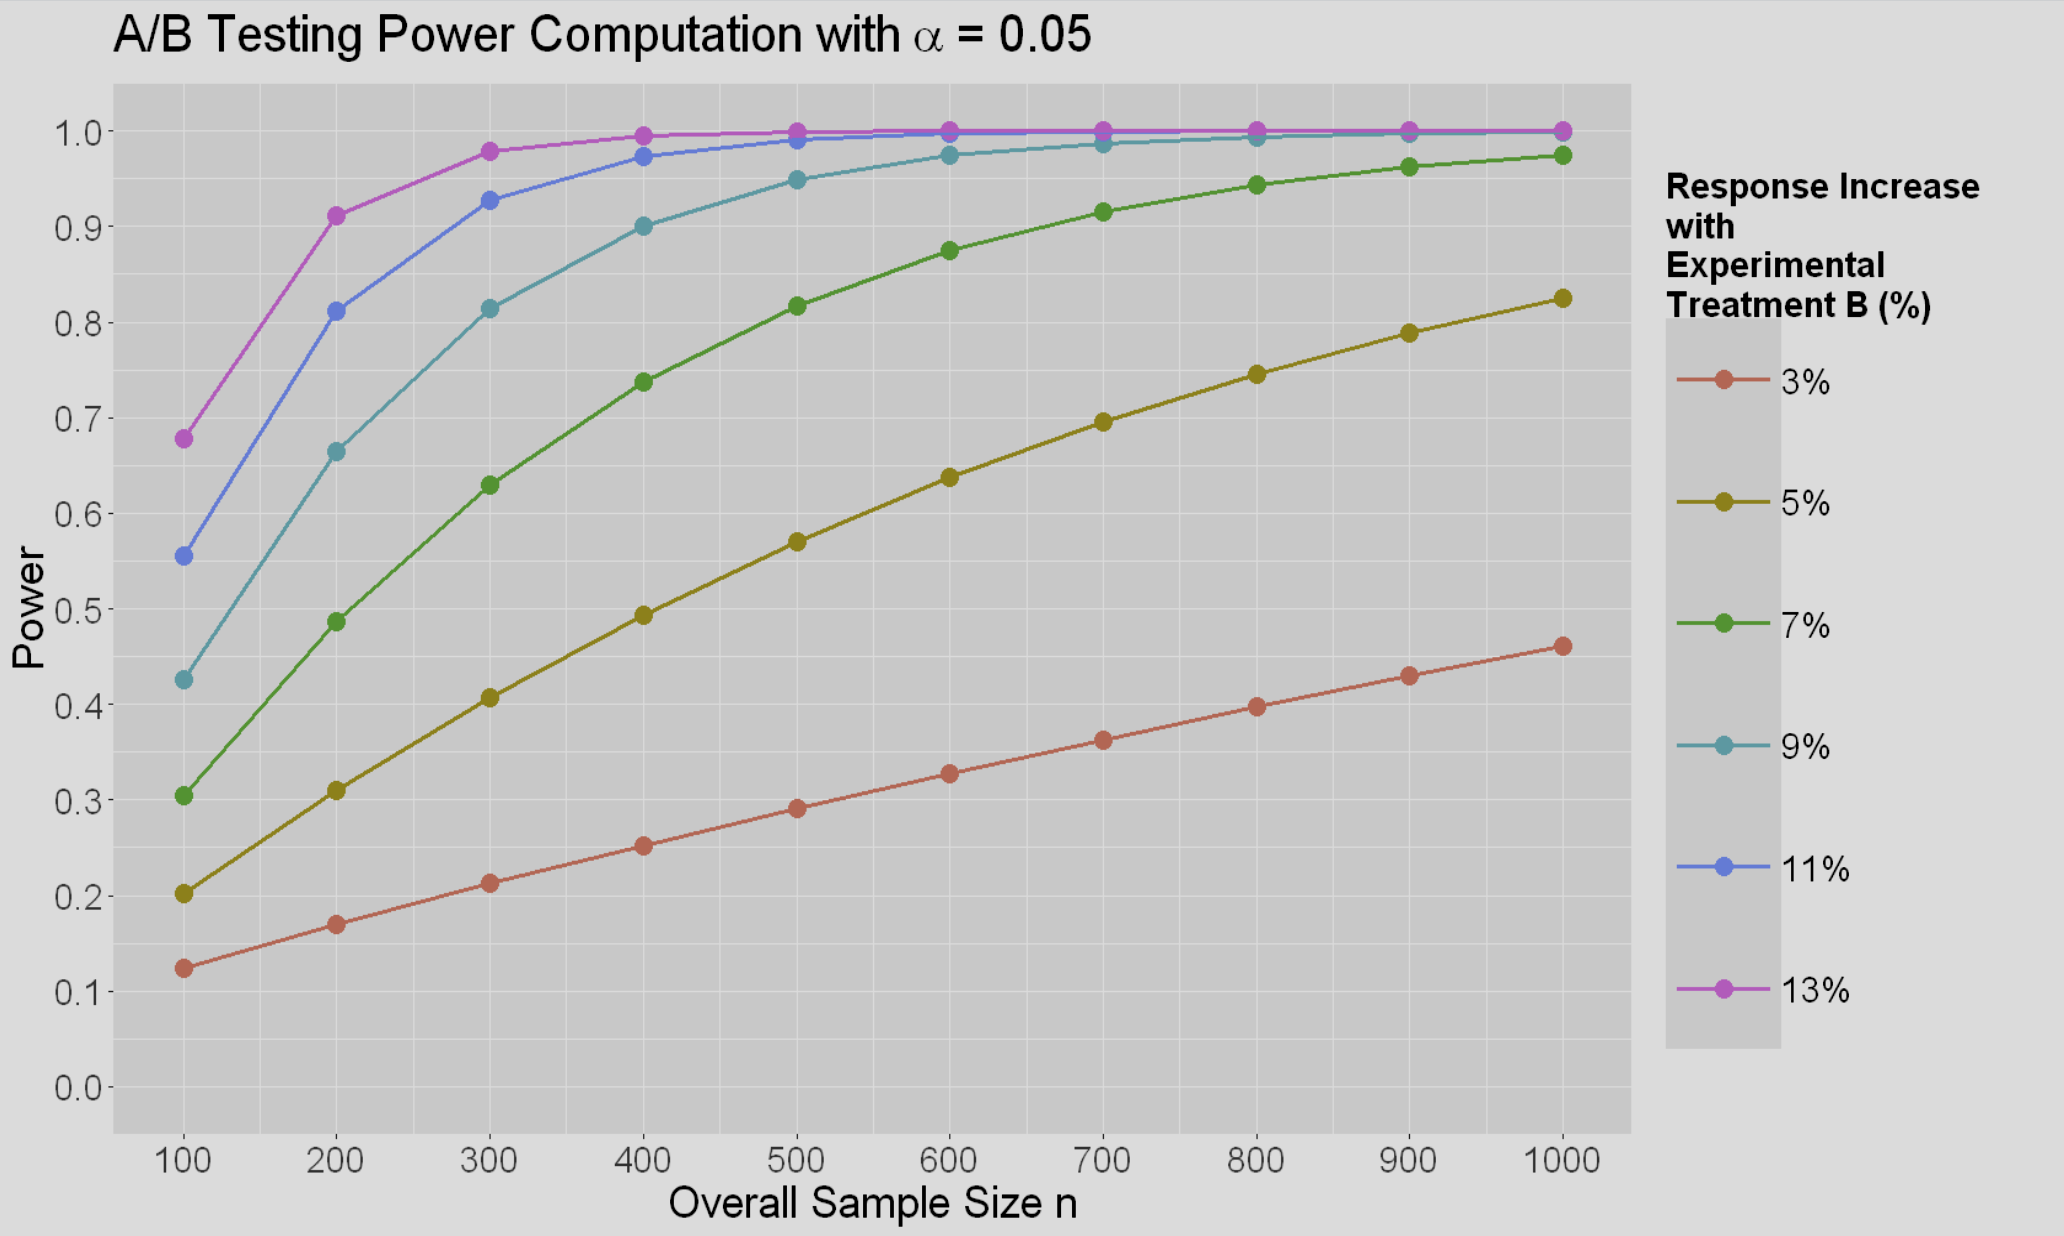
\includegraphics[width=0.50\linewidth, height=2cm]{power-1.png}
  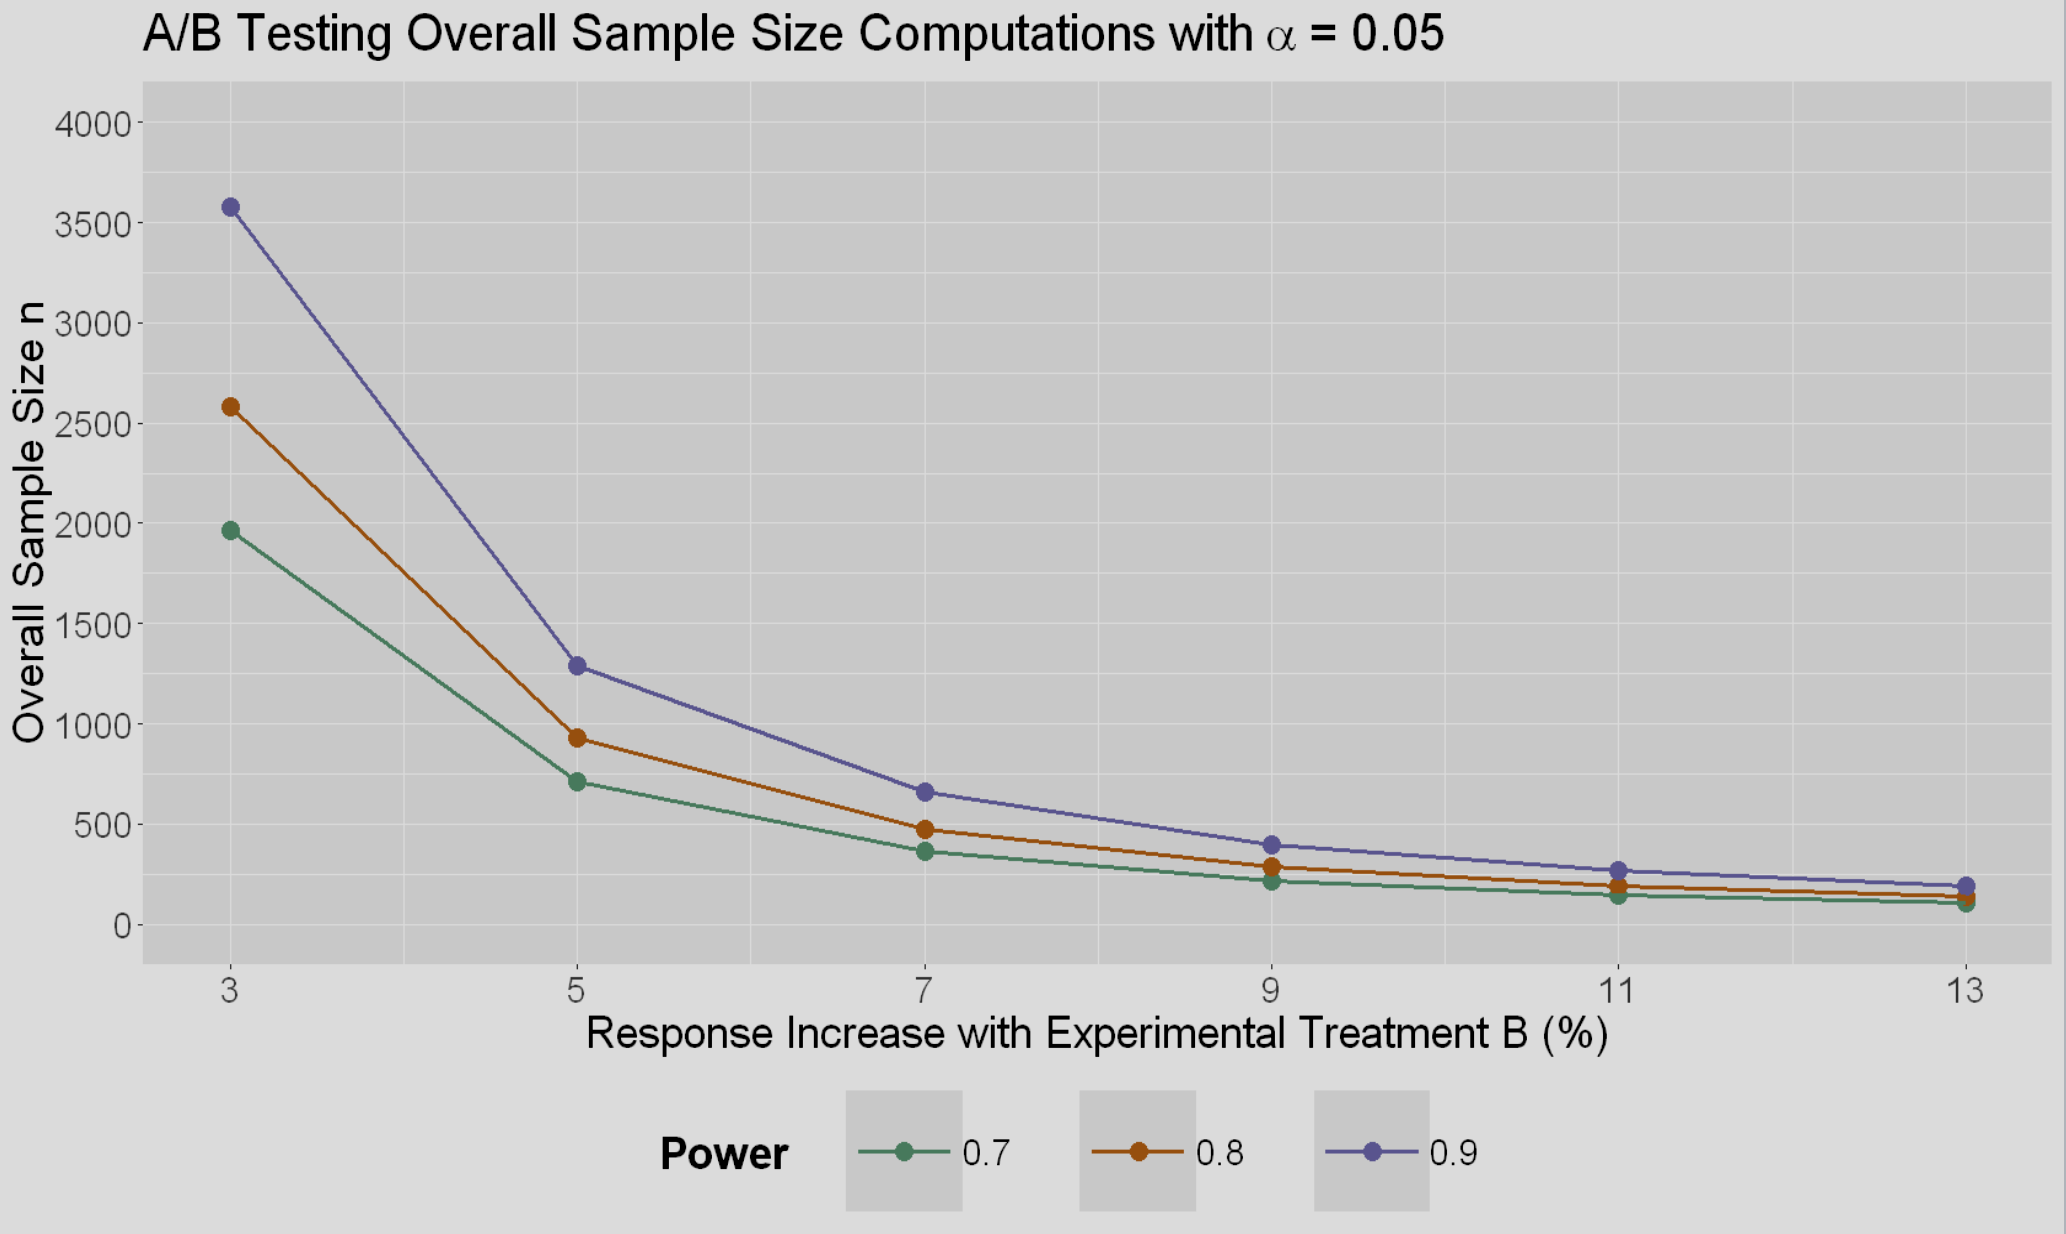
\includegraphics[width=0.50\linewidth, height=2cm]{power-2.png}
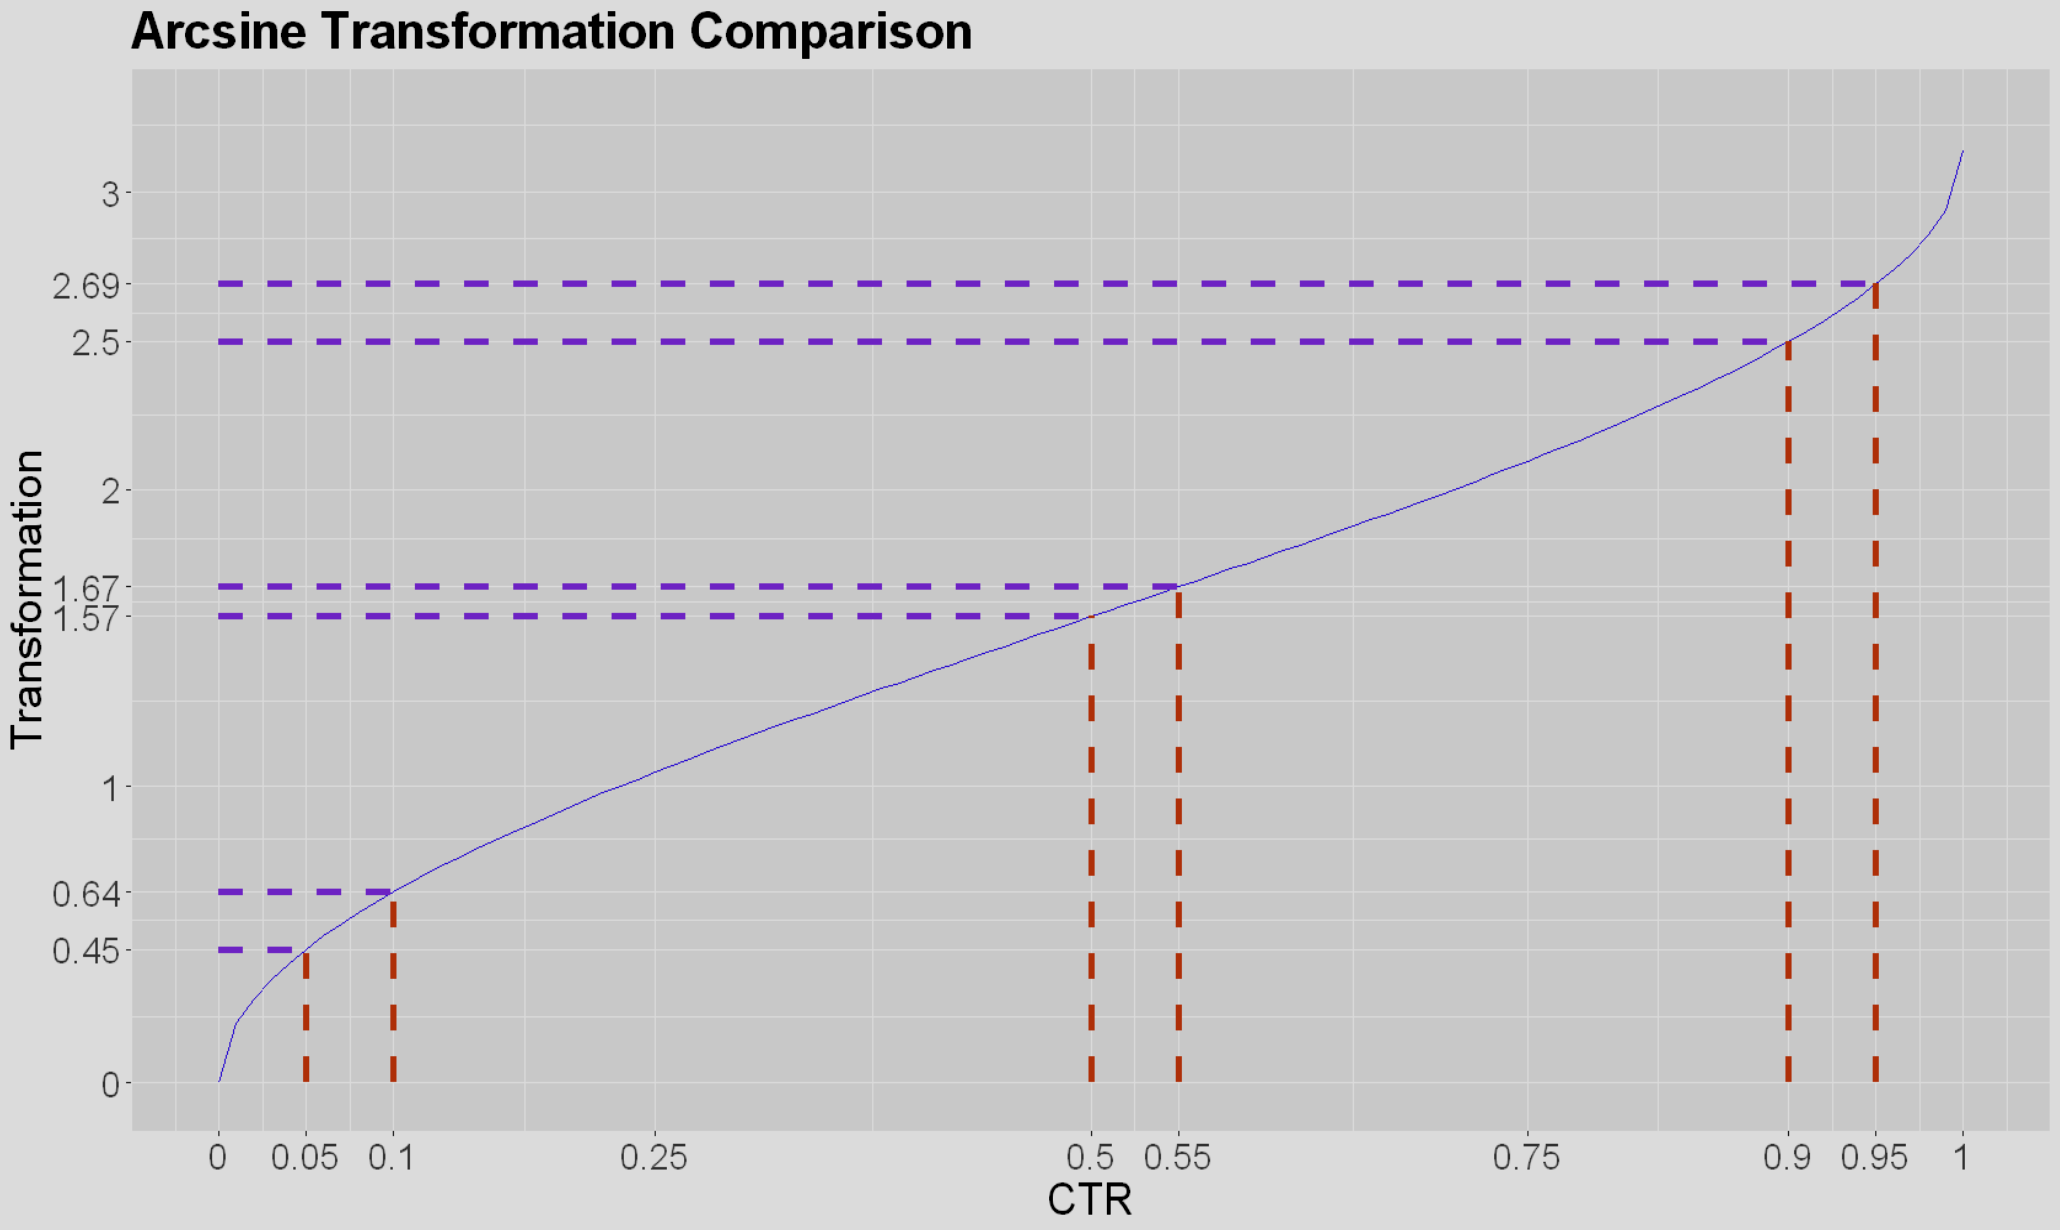
\includegraphics[width=0.30\linewidth, height=2cm]{arcsine.png}
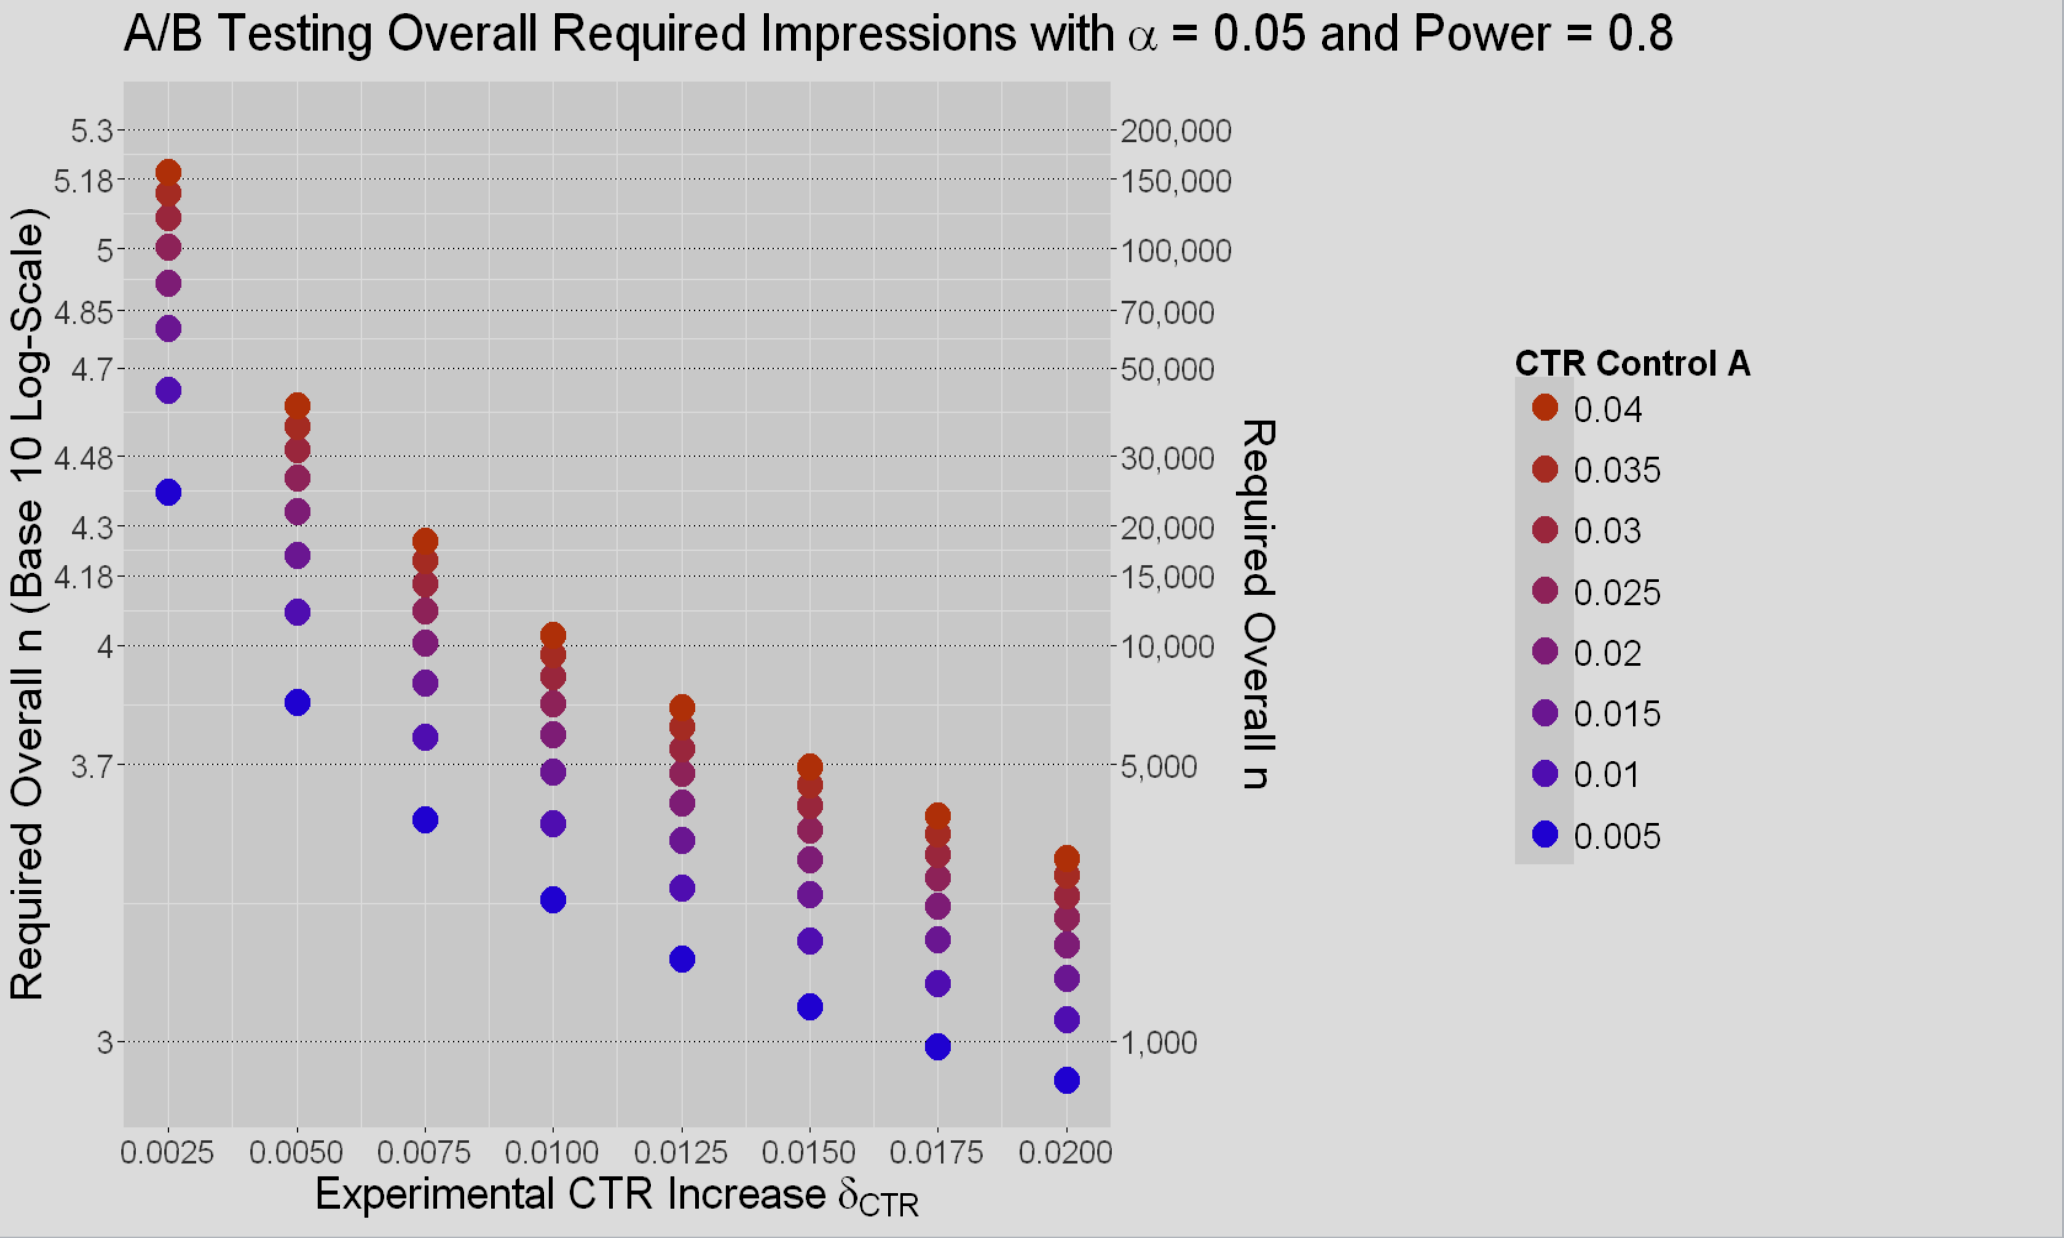
\includegraphics[width=0.30\linewidth, height=2cm]{ctr-delta.png}
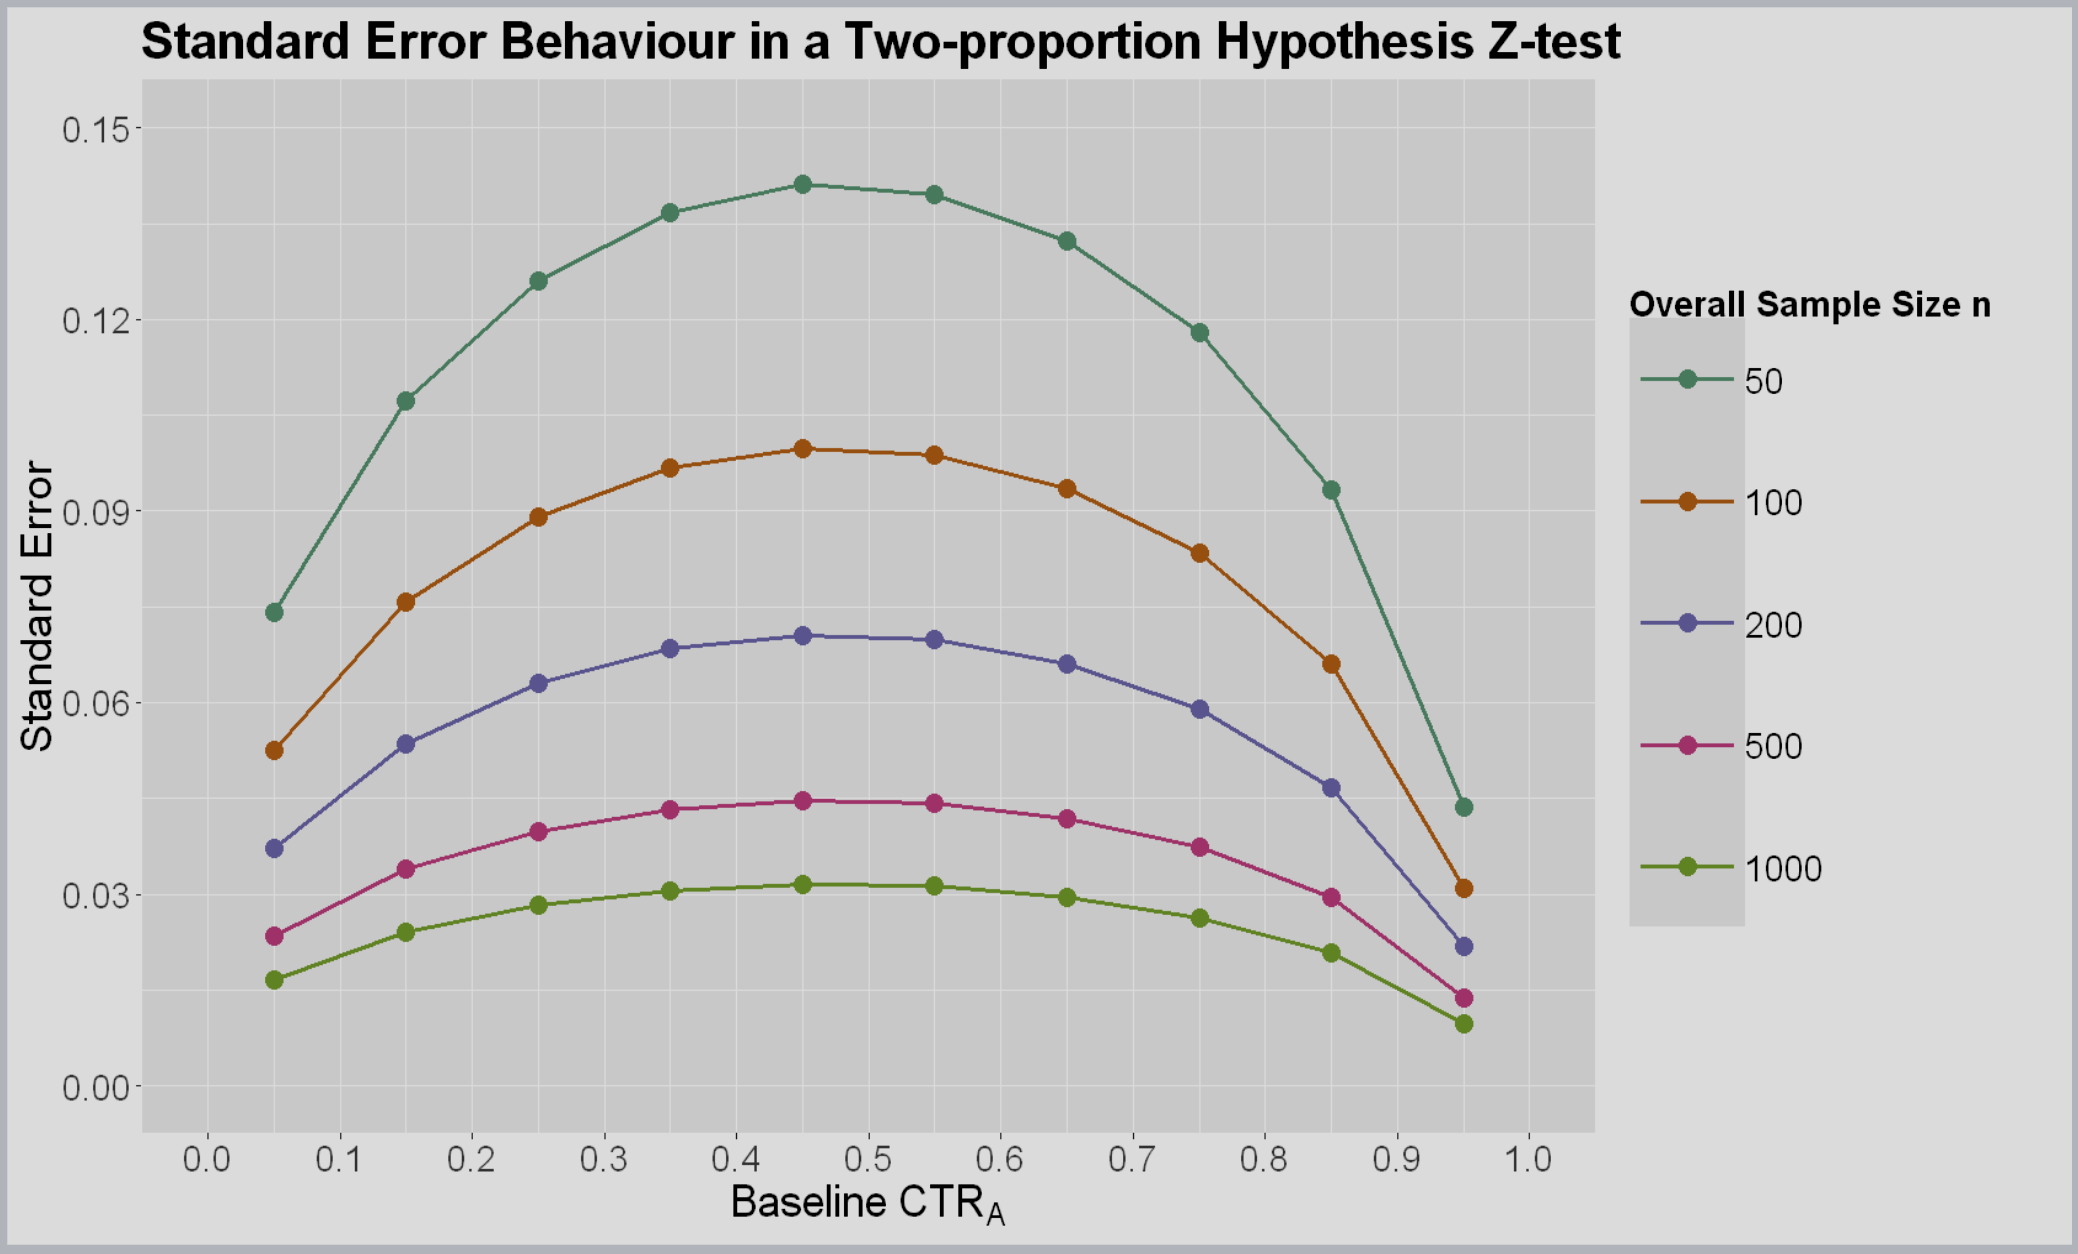
\includegraphics[width=0.30\linewidth, height=2cm]{z-test.png}
  \section{Early Stopping and Peeking}
  \subsection{Aggressive Peeking}
  \smalltext{
  Peeking involves accessing data in real-time before reaching $n_{max}$.
  \begin{itemize}
      \item \textbf{Type I Error Inflation}: Aggressive peeking (checking every visitor) \textbf{severely inflates} the Type I error rate (up to $\sim$25\% for $\alpha=0.05$) because it gives the test multiple chances to cross the significance threshold by chance.
      \item \textbf{Power Loss}: While it can stop early for large effects, aggressive peeking causes a \textbf{power decrease} if the true CTR increase is small
  \end{itemize}
  }
  
  \subsection{Principled Peeking}
  \smalltext{
  Principled peeking uses a fixed number of peeks ($m$) and the \textbf{Bonferroni correction} ($\alpha/m$).
  \begin{itemize}
      \item \textbf{Error Control}: The $\alpha/m$ adjustment prevents the inflation of false positives seen in aggressive peeking .
      \item \textbf{Optimal Strategy}: 2 principled peeks are often considered ideal; increasing peeks beyond this can significantly \textbf{reduce power}.
  \end{itemize}
  }
  
  \smalltext{
  \setlength{\tabcolsep}{4pt} 
  \renewcommand{\arraystretch}{1} 
  \begin{tabular}{|p{2.2cm}|c|c|}
  \hline
  \textbf{Decision} & \textbf{$H_0$ is True} & \textbf{$H_0$ is False} \\ \hline
  \textbf{Fail to Reject} & Correct (TN) & Type II Error (FN / $\beta$) \\ \hline
  \textbf{Reject $H_0$} & Type I Error (FP / $\alpha$) & Correct (TP / Power) \\ \hline
  \end{tabular}
  }

  \section{Observational Studies \& Confounding}
\subsection{Causal Inference Challenges}
\smalltext{
In observational studies, the researcher lacks control over the variable of interest $X$, as subjects often self-select into treatment groups. Because randomization is absent, these studies cannot automatically eliminate the effects of confounding variables, making causal interpretation difficult. The general strategy involves recording potential confounders during data collection and incorporating them into the analysis while tempering causal claims. Data science applications, such as pharmaco-epidemiology, utilize massive healthcare databases to estimate what would occur in a randomized trial setting.

\textbf{Naive vs. Adjusted}: The "direction" of an effect can flip in an adjusted model. This happens because the naive model mixes the relationship between X, Y, and the confounder. Adjusting allows the model to interpret the effect conditional on the confounder.
}

\section{Statistical Metrics for Binary Outcomes}
\subsection{Log-Odds and Odds Ratios}
\smalltext{
Binary logistic regression utilizes the log-odds, defined as the natural logarithm of the ratio of success probability to failure probability. The Odds Ratio (OR) measures the association or potential causation between an exposure $X$ and an outcome $Y$. An $OR = 1$ indicates the exposure does not affect the outcome odds, while an $OR > 1$ suggests the exposure is associated with higher odds of the outcome. The Western Collaborative Group Study (WCGS) uses these metrics to assess if Type A behavior patterns lead to higher odds of coronary heart disease (CHD).
}

\begin{lstlisting}[language=R]
initial_bin_log <- glm(chd69 ~ dibpat, data = training_data, family = "binomial")
tidy(initial_bin_log, conf.int = 0.95)
detach(training_data)
training_data <- training_data %>%
  mutate(bmi_bins = cut(bmi, breaks = c(min(bmi), quantile(bmi, (1:3) / 4), max(bmi)), include.lowest = TRUE))
levels(training_data$bmi_bins)
bin_log_model <- glm(chd69 ~ dibpat + age_bins + bmi_bins + smoke, 
                     data = training_data, family = "binomial")
tidy(bin_log_model, conf.int = 0.95) %>% 
  mutate(exp.estimate = exp(estimate)) %>%
  mutate_if(is.numeric, round, 3)
p_values <- c(anova(bin_log_model, triple_bin_log_model, test = "LRT")$`Pr(>Chi)`[2]) # Storing p-value
\end{lstlisting}

\section{Stratification and Modeling Strategies}
\subsection{Adjusting for Multiple Confounders}
\smalltext{
Stratification involves "slicing" data based on confounding variables, such as age bins, to identify stratum-specific effects. However, stratifying by multiple variables (e.g., age, smoking, and BMI) can lead to very small subsamples, resulting in insufficient data for estimation and high uncertainty. An overall Binomial Logistic Regression serves as a more efficient approach, acting as a "proxy for blocking" by including confounders as standalone regressors. This model assumes a simple structure for log-OR variation across strata and the absence of interactions between the exposure and confounders.
}

\section{Model Selection and Assumptions}
\subsection{Testing and Causal Reasoning}
\smalltext{
Causal inference from regression models requires meeting strong assumptions, including the inclusion of all relevant confounders and the lack of unobserved confounding. Model selection often employs Likelihood Ratio Tests (LRT) to compare nested models, such as testing for the necessity of interaction terms. While multiple testing corrections like Bonferroni manage significance levels, they can be overly strict and may exclude genuine confounders that are causally relevant. Therefore, model selection should combine statistical testing with subject-matter knowledge about the data-generating process.
}

\section{Sampling Schemes \& Proxy Ground Truth}
\subsection{Simulation Frameworks}
In frequentist statistics, access to the population's \textbf{ground truth} is often impossible. Simulation serves as a proxy ground truth by using a representative dataset to fit a model, which then generates artificial outcomes ($Y$) based on estimated regression coefficients and design matrices. This approach allows researchers to assess the accuracy and precision of different sampling designs before implementation. Causal inference in these models relies on controlling for confounders ($C_j$) to assume a common effect of $X$ over $Y$ across all subjects.

\textbf{Proxy vs. Synthetic}: Proxy ground truth (built from real surveys) preserves realistic associations between X, Y, and confounders, whereas simple synthetic data often misses these complexities and yields overly idealized performance estimates.

\section{Comparing Observational Schemes}
\subsection{CS, CC, and CO Temporalities}
Three primary schemes exist: 
1. \textbf{Cross-Sectional (CS)} is contemporaneous, taking a simple random snapshot of the population. 
2. \textbf{Case-Control (CC)} is retrospective, sampling half from those with the outcome ($Y=1$, cases) and half from those without ($Y=0$, controls). 
3. \textbf{Cohort (CO)} is prospective, sampling based on exposure ($X$) and tracking outcomes over time. While CS is ideal for early research, CC is significantly more efficient when the outcome is rare, offering higher power and lower RMSE.

\begin{lstlisting}[language=R]
# Simulating outcomes for Proxy Ground Truth
pred_prob <- function(logit) {exp(logit) / (1 + exp(logit))}
sim_pop$chd69 <- rbinom(n = nrow(sim_pop), size = 1,
prob = pred_prob(logit = model_matrix %*% coefs))
# Case-Control Sampling (Retrospective)
CC_subjects <- c(
sample(which(sim_pop$chd69 == "0"), size = n / 2),
sample(which(sim_pop$chd69 == "1"), size = n / 2))
\end{lstlisting}

\section{Case-Control Efficiency}
\subsection{Case:Control Ratios and Precision}
The efficiency of Case-Control studies is analyzed via a modified power analysis focusing on the \textbf{Standard Error (SE)} of the log-OR estimate. In populations where the event is rare (e.g., $<10\%$), \textbf{oversampling cases} ($Y=1$) and undersampling controls ($Y=0$) acts as a winning strategy for precision. Precision increases as the Case:Control ratio reaches or slightly exceeds 1.0, particularly when the estimated log-OR is low. The SE is minimized as the cell frequencies in the contingency table become more balanced through this strategic oversampling.

\section{Matched Case-Control Studies}
\subsection{Matching and McNemar Analysis}
Matched Case-Control (CC) sampling involves selecting $n/2$ cases ($Y=1$) and then finding $n/2$ controls ($Y=0$) that exactly match each case's confounding strata ($C_j$). This design allows for stronger causal claims. Because pairs are dependent, Binary Logistic Regression via \code{glm()} can lead to the "sparse data problem". Instead, the \textbf{McNemar test} is used, focusing on \textbf{discordant pairs}: $n_{1,0}$ (Case $X=1$, Control $X=0$) and $n_{0,1}$ (Case $X=0$, Control $X=1$). The OR is estimated as $n_{1,0}/n_{0,1}$. Simulation shows matched CC has \textbf{smaller BIAS and RMSE} than unmatched CC at small sample sizes (e.g., $n=100$).

\textbf{Why not glm?}: Classical \code{glm()} assumes independent observations. Matched data has a pairing structure (dependency). Using \code{glm()} on matched data leads to the "sparse data problem".

\begin{lstlisting}[language=R]
# Estimating log-OR for matched samples
logOR_est <- log(n10) - log(n01)
logOR_se <- sqrt(1/n10 + 1/n01)

# Ordinal Contrasts
options(contrasts = c("contr.treatment", "contr.sdif"))
\end{lstlisting}

\section{Ordinal Regressors}
\subsection{Polynomial and Successive Contrasts}
Ordinal regressors are categorical factors with ordered levels (e.g., discount percentages). Rather than standard dummy coding, \textbf{contrasts} (vectors summing to zero) provide deeper insight.
\begin{itemize}
    \item \textbf{Polynomial Contrasts}: Decompose data into Linear (L), Quadratic (Q), and Cubic (C) trends. Useful for testing if a specific trend exists in the ordered levels.
    \item \textbf{Successive Differences (\code{contr.sdif})}: Directly compare the mean of one level to its immediate predecessor (e.g., $L_2 - L_1$). These are often more interpretable for specific statistical inquiries.
\end{itemize}

\textbf{Decision Strategy}:
\begin{itemize}
    \item \textbf{CS}: Quick preliminary evidence.
    \item \textbf{CC}: Efficient for \textbf{rare outcomes} (start with diseased).
    \item \textbf{CO}: Efficient for \textbf{rare exposures} (start with exposed).
\end{itemize}

\subsection{Experimental vs. Observational}
\textbf{Experimental}: Full control over treatments. Randomization eliminates confounders. Blocking ensures precision by grouping homogeneous units before randomizing.

\textbf{Observational}: No randomization. Uses stratification or matching via confounders to approximate causal comparisons. Analysis must reflect collection: CS (simple random), CC (retrospective, rare outcomes), CO (prospective).

\end{multicols}
\end{document}